\documentclass{article}
\usepackage{fancyhdr}
\usepackage{lipsum}  
\usepackage{listings} 
\usepackage{xcolor}   
\usepackage{amsmath}
\usepackage{enumitem}
\usepackage{graphicx}
\usepackage{caption}
\usepackage{verbatim}

% Define macros for title and author
\newcommand{\thetitle}{STAT 641 \\ Homework 7}
\newcommand{\theauthor}{Keegan Smith}

\title{\thetitle}
\author{\theauthor}

\pagestyle{fancy}
\fancyhf{}  % Clear all header and footer fields
\fancyhead[L]{\nouppercase{\rightmark}}
\fancyhead[C]{\thetitle}  % Title in the center
\fancyhead[R]{\theauthor}  % Your name on the right

\lstset{ %
  backgroundcolor=\color{lightgray},   % choose the background color
  basicstyle=\ttfamily\small,          % size of fonts used for the code
  keywordstyle=\color{blue},           % color for keywords
  commentstyle=\color{green},          % color for comments
  stringstyle=\color{red},             % color for strings
  numbers=left,                        % where to put the line-numbers
  numberstyle=\tiny\color{gray},       % style for line-numbers
  stepnumber=1,                        % the step between two line-numbers
  numbersep=5pt,                       % how far the line-numbers are from the code
  frame=single,                        % adds a frame around the code
  rulecolor=\color{black},             % frame color
  breaklines=true,                     % automatic line breaking
  breakatwhitespace=false,             % automatic breaks should only happen at whitespace
  showspaces=false,                    % don't show spaces in the code
  showstringspaces=false,              % don't show spaces in strings
  showtabs=false,                      % don't show tabs in the code
}

\begin{document}

\maketitle
\section*{Problem 1}
\begin{enumerate}
\item The rejection region is defined as: \\
\[
R = {X : T(X) > C}
\]
where $T(X)$ is the distribution of the test statistic $X$. \\
Since $Y$ is normally distributed we can use the test statistic: \\
\[
T = \frac{\sqrt{n}(\bar{Y} - \mu_o)}{\sigma}
\]
Substituting our values we get: \\
\begin{align*}
T &= \frac{\sqrt{36}(\hat{\mu} - 10)}{\hat{\sigma}} 
\end{align*}
And we have the critical value (obtained from the table): \\
\begin{align*}
t_{.025, 35} &= 2.0315
\end{align*}
Thus our rejection region is: \\
\[
R = {(\hat{\mu}, \hat{\sigma}) : \frac{\sqrt{36}(\hat{\mu} - 10)}{\hat{\sigma}} > 2.0315}
\]
\item The power function is: \\
\[
\gamma(\mu) = G(-t_{.025}) + 1 - G(t_{t_{.025}}) \\
\]
Where $G$ is the cdf of the students $T$ distribution centered at:
\[
T = \frac{\sqrt{36}(\mu - 10)}{.27}
\]
with $df = 35$. \\
Graphing this function in R: \\
\begin{figure}[htbp]
  \centering
  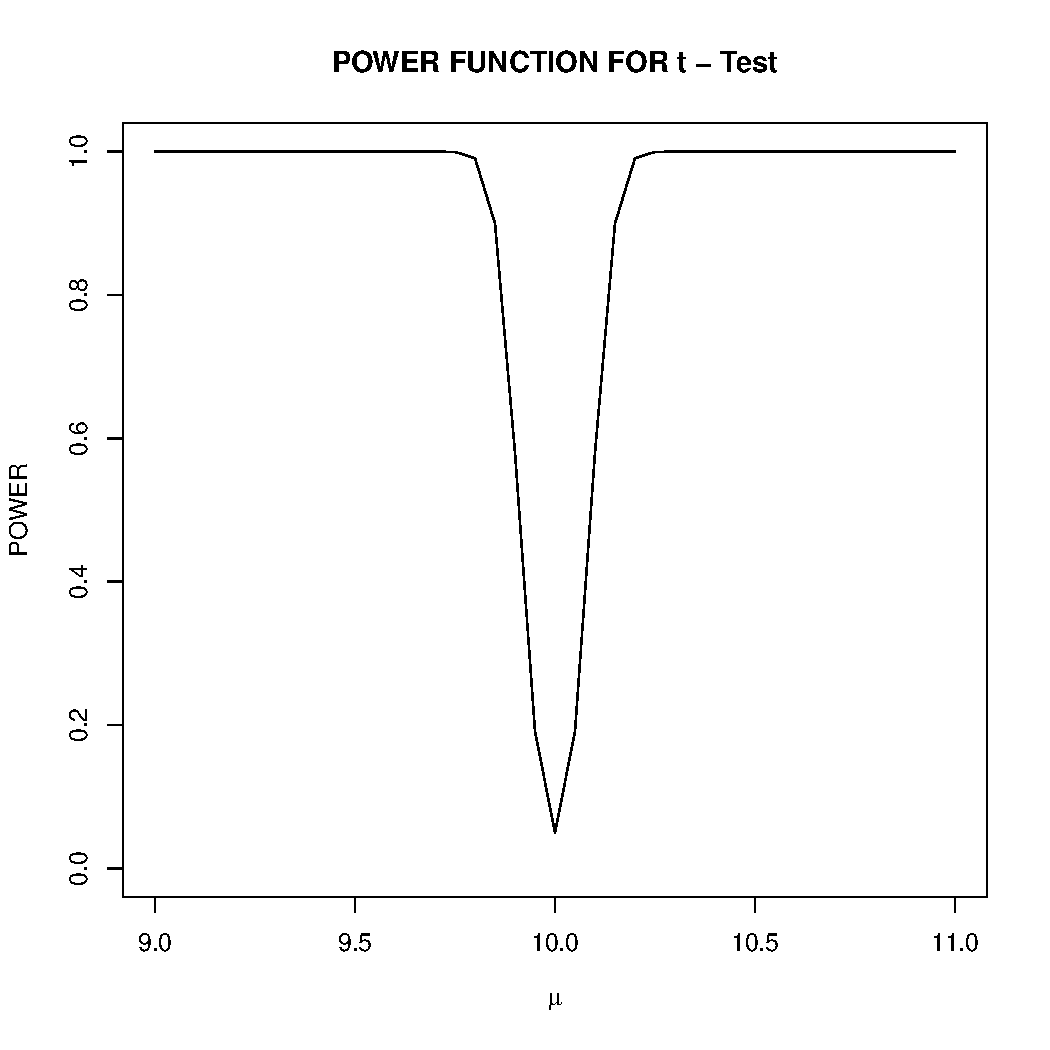
\includegraphics[width=0.8\textwidth]{Rplots.pdf}
\end{figure}
\newpage
The R code is: \\
\begin{verbatim}
n = 36
df = n-1
muo = 10
sigma = .27
mu = seq(9,11,.05)
delta = sqrt(n)*(mu-muo)/sigma
power = 1-pt(qt(.975,df),df,delta) + pt(qt(.025, df), df, delta)
#par(lab=c(15,20,4))
plot(mu,power,type="l",ylim=c(0,1),xlab=expression(mu),
ylab="POWER")
title("POWER FUNCTION FOR t - Test")
out = cbind(mu,delta,power)
\end{verbatim}
The sample mean is 10, so our $T$ statistic is 0, thus $G$ is centered at 0, so: \\
\begin{align*}
\gamma(\mu) &= G(-t_{.025}) + 1 - G(t_{.025}) \\
&= .025 + 1 - .975 \\
&= .05
\end{align*}
\item To determine the sample size, we have $\alpha = .05$, $\beta = .2$, and $\phi = \frac{.2}{.27} = 0.7407$. From the table $A11$, this gives us a sample size of $13$. \\
\end{enumerate}
\section*{Problem 2}
\begin{enumerate}
\item The null hypothesis is $\mu \geq 5$, with the alternative hypothesis being $\mu < 5$. \\
$\sigma$ is unkown, so we will be using t testing. \\
We know that: $n = 20$, $\hat{\mu} = 4.2$, $S = 1.2$, and $\alpha = .05$, so we have the T statistic: \\
\[
T = \frac{\sqrt{20}(4.2 - 5)}{1.2} = -2.98142396999972
\]
the t critical value is: \\
\[
t_{.05} = -1.729
\]
(from the table). \\
Since $T < t_{.05}$, we reject the null hypothesis. We also have the p-value for $T$ which is approximately $.005 < .05$ from the table. \\
\item The probability that the test will be able to detect that the real mean is 4.1 or less can be given by the power function [ ]
\[
\gamma(\mu) = G(-t_{.05})
\]
where $G$ is the cumulative t distribution centered at $\delta = \frac{\sqrt{20}(4.1 - 5)}{1.2}$ with $df = 19$. This can be solved with R: \\
\begin{verbatim}
result = pt(-qt(.05, 19), 19, 0.3727)
\end{verbatim}
which yields a power of 0.9006489
\item For sample size estimation we know: $\alpha = .05$, $\beta = .1$, and $\phi = \frac{|4.4 - 5|}{1.2} = .5$. From the table this gives us 44
\end{enumerate}
\section*{Problem 3}
\begin{enumerate}
\item We will assume the population distribution is normal, since this is a manufacturing process. \\
The null hypothesis is that $\sigma \geq 1$, the alternative hypothesis is that $\sigma < 1$. We can calculate the test statistic: \\
\begin{align*}
TS &= \frac{(n - 1) * S^2}{\sigma_o} \\
&= \frac{19 * .8458^2}{1} \\
&= 13.5922
\end{align*}
we can determine the critical value with: \\
\begin{align*}
t_{.05} &= \chi_{19, .95}^2 \\
&= 10.117
\end{align*}
The test statistic is not less than the critical value, thus we fail to reject the null hypothesis. \\
\item We have the power function: \\
\begin{align*}
power &= G(\frac{\sigma_o^2}{\sigma_1^2}\chi^2_{n - 1, 1 - \alpha}) \\
&= G(10.117) \\
&= .05 \\
\end{align*}
so the type II error rate for $\sigma_1 = 1$ is $1 - .05 = .95$. For $\sigma_1 = .9$: \\
\begin{align*}
power &= G(\frac{\sigma_o^2}{\sigma_1^2}\chi^2_{n - 1, 1 - \alpha}) \\
&= G(\frac{1^2}{.9^2}\cdot 10.117) \\
&= G(12.4901) \\
&= 0.1363781
\end{align*}
so the type II error is 0.8636219. For $\sigma_1 = .8$: \\
\begin{align*}
power &= G(\frac{\sigma_o^2}{\sigma_1^2}\chi^2_{n - 1, 1 - \alpha}) \\
&= G(\frac{1^2}{.8^2}\cdot 10.117) \\
&= G(15.81) \\
&= 0.32994
\end{align*}
so the type II error is 0.67006. For $\sigma_1 = .7$: \\
\begin{align*}
power &= G(\frac{\sigma_o^2}{\sigma_1^2}\chi^2_{n - 1, 1 - \alpha}) \\
&= G(\frac{1^2}{.7^2}\cdot 10.117) \\
&= G(20.6469) \\
&= 0.6433
\end{align*}
so the type II error is .3567. For $\sigma_1 = .6$: \\
\begin{align*}
power &= G(\frac{\sigma_o^2}{\sigma_1^2}\chi^2_{n - 1, 1 - \alpha}) \\
&= G(\frac{1^2}{.6^2}\cdot 10.117) \\
&= G(28.1027) \\
&= 0.918528
\end{align*}
so the type II error is .08147. \\
\item The bound for the upper 90\% CI is given by: \\
\begin{align*}
CI &= \frac{\sqrt{n - 1} \cdot S}{\sqrt{X^2_{1 - \alpha, n - 1}}} \\
&= \frac{\sqrt{19} \cdot .8458}{\sqrt{X^2_{.9, 19}}} \\
&= \frac{\sqrt{19} \cdot .8458}{\sqrt{11.651}} \\
&= 1.0801
\end{align*}
This aligns with my results in part 1 since 1 is included the in the CI. 
\end{enumerate}
\section*{Problem 4}
\begin{enumerate}
\item $S_+ = 5$, so we have: \\
\[
p = G(5, 20, .5) = .021
\]
where G is the cdf of the binomial distribution with $p = .5$, $n = 20$, and $x = 5$. \\
.021 < .05, so we reject the null hypothesis. \\
\item Following the procedure in handout 12, we find that $W_+ = 68.5$ and $W_- = 141.5$. \\
We find from psignrank(68.5, 20, TRUE) that $p = 0.09467411 < .05$ so we reject the null hypothesis. 
\item We can invert the wilcox test to find an upper bound. We need to find the first value where we would reject the null hypothesis if it were the sample median. We will do a binary search: \\
Trying $H_0 = 10.07$: \\
$W_+ = 100, W_- = 90$ \\
psignrank(100, 20, TRUE)  = 0.4347439 > .1, so fail to reject. \\
Trying $H_0 = 10.93$: \\
$W_+ = 20, W_- = 170$ \\
psignrank(20, 20, TRUE) = 0.0003538132, so reject. \\
Trying $H_0 = 10.15$: \\
$W_+ = 79.5$ \\
psignrank(79.5, 20, TRUE) = 0.1841383 > .1 so fail to reject. \\
Trying $H_0 = 10.24$: \\
$W_+ = 78$ \\
psignrank(78, 20, TRUE) = 0.1649914 > .1 so fail to reject. \\
So the 90\% upper bound is 10.24. 
\end{enumerate}
\section*{Problem 5}
\begin{enumerate}
\item idk, just use wald CI I guess: \\
\begin{align*}
CI &= \hat{p} \pm Z_{.025}\frac{\sqrt{\hat{p}(1 - \hat{p})}}{\sqrt{n}} \\
&= .65 \pm 1.96 \frac{\sqrt{.65(1 - .65)}}{\sqrt{200}} \\
&= 0.583895385940163, 0.716104614059837
\end{align*}
\item we have the test statistic: \\
\begin{align*}
TS &= \frac{.65 - .6}{\sqrt{\frac{.65 \cdot .35}{200}}} \\
&= 1.4824986333222026
\end{align*}
the p value is: \\
\[
p = 1 - pnorm(1.48) = 0.06943662
\]
greater than $\alpha$ so fail to reject. \\
\item so we have the power function: \\
\[
power = 1 - pnorm(Z_\alpha \cdot \sqrt{\frac{p_o(1 - p_o)}{p_1(1 - p_1)} + \frac{\sqrt{n}(p_o - p_1)}{\sqrt{p_1(1 - p_1)}}})
\]
This is the power function implemented in R: \\
\begin{verbatim}
power_from_formula <- function(n, p0, p1, alpha = 0.05) {
z_alpha <- qnorm(1 - alpha)
inside_sqrt <- 
  p0*(1 - p0) / (p1*(1 - p1)) +
  ( sqrt(n) * (p0 - p1) ) / sqrt(p1*(1 - p1))
1 - pnorm( z_alpha * sqrt(inside_sqrt) )
}
\end{verbatim}
When plugging in our values, we get: \\
0.001178664 \\
0.05 \\
0.4180287 \\
0.9078522 \\
0.9988094 \\
for .55, .6, .65, .7, .75 respectively. \\
\end{enumerate}
section*{Problem 6}
\begin{enumerate}
\item b \\
\item c \\
\item d \\
\item a \\
\item b \\
\item c \\
\end{enumerate}
\end{document}